\chapter{Grundlagen}
\label{chap:grundlagen}

In diesem Abschnitt meiner Arbeit, möchte ich zu erst die nötigen Grundlagen behandeln, um ein Basiswissen für die folgenden Kapitel sicherzustellen.\\
Da sich die Arbeit hauptsächlich um den Bildmerkmal Algorithmus \textbf{Histogram of Oriented Gradients} Algorithmus dreht, fange ich mit diesem an.
\section{Histogram of Oriented Gradients}
\label{sec:grundlagenhog}
Wie gerade erwähnt ist der \textbf{HOG} ein Bildmerkmal Algorithmus, der sich gegen bekannte Algorithmen (z.B. SIFT) bestens schlägt und dabei  effizienter arbeitet. Entwickelt und vorgestellt wurde der Algorithmus von Navneet Dalal und Bill Triggs im Paper $Histograms~of ~oriented~Gradients~for~Human~Detection$ \cite{dalal:inria-00548512} veröffentlicht.\\
Grundlegend funktioniert der Algorithmus durch das Beschreiben von Verläufen. Diese Informationen werden in ein geeignetes Format gebracht um anschließend das betrachtete Bild zu klassifizieren. Wie in der ursprünglichen Arbeit, wird in dieser Arbeit erkannt ob ein Mensch in  einem Bild vorhanden ist.\\
Den gesamten Ablauf kann man in Abbildung 2.1 sehen. Da einige Schritte für das Verständnis nicht erforderlich sind, werde ich nur einen Teil dieser erklären.

\begin{figure}[htbp]\centering 
	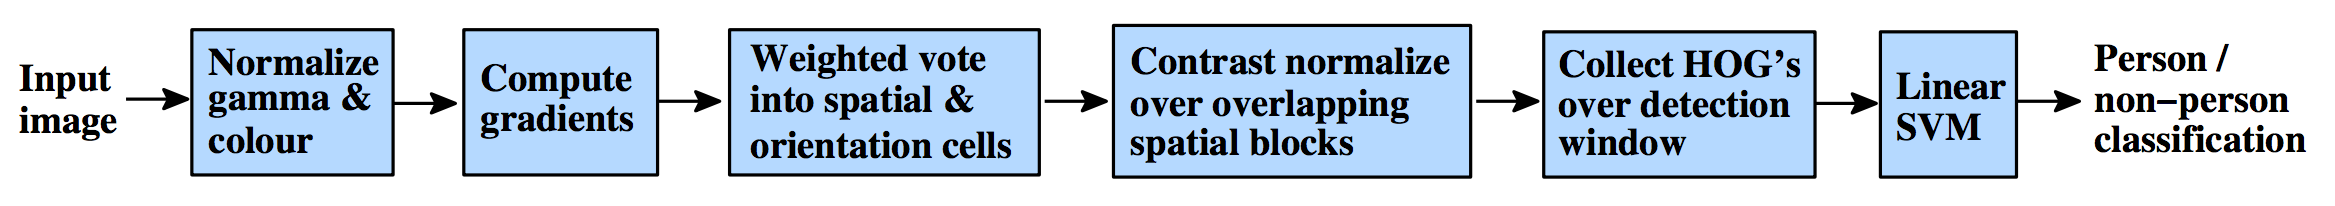
\includegraphics[width=1\linewidth]{./pics/feature extraction chain.png} 
	\caption{Ablauf der Klassifizierung von Bildmerkmalen
	\cite{dalal:inria-00548512}}\label{fig:grundlagen_feature_extraction_chain}\end{figure}

Die wichtigsten Bestandteile werde ich im Folgenden erklären.

\subsection{Gradienten-Vektoren}

Wie der Name zu erkennen gibt, betrachtet der \textbf{HOG}-Algorithmus die Gradienten eines Bildes. Beschrieben werden Gradienten durch Vektoren:

$$
\vec{g}=\begin{pmatrix}
	g_x \\
	g_y
\end{pmatrix}
$$

Um die Elemente $g_x$ und $g_y$ zu berechnen, gibt es einige mögliche Filter. Laut $Dalal$ und $Triggs$ \cite[S.5]{dalal:inria-00548512} funktioniert der simple Filter

$$
\vec{x}=\begin{pmatrix}
	-1 & 0 & 1
\end{pmatrix}
$$
bzw.
$$
\vec{y}=\begin{pmatrix}
	-1 \\
	0 \\
	1
\end{pmatrix}
$$
am besten.
Diese Filter werden auf jeden Bildpunkt im Bild angewandt. Somit ergibt sich die Berechnung von $g_x$ und $g_y$ zu:
\begin{equation*}
	g_{x_k}=-x_{k-1}+x_{k+1} \\
	g_{y_k}=-y_{k-1}+y_{k+1}
\end{equation*}

Dabei ist $x_k$ der betrachtete horizontale Bildpunkt und $y_k$ ist der betrachtete vertikale Bildpunkt.\\
Jedoch aufgepasst, man muss beachten, dass bei einem Farbbild $g_x$ und $g_y$ für jeden Farbkanal berechnet werden müssen. Zusätzlich verhält sich die Berechnung am Rand des Bildes etwas anders.
Wie in der Abbildung ... dargestellt, wird der Wert des Bildpunktes am Rand für die Berechnung einfach wiederholt.


\begin{figure}[!h]
\centering

\begin{tikzpicture}[
        x=1.5cm,
        y=1.5cm]
  
\draw[thick] (0,0)--(4.4,4.4); % l'axe des abscisses
\draw[thick] (1,0)--(6,0) ;
\draw[thick] (0,1)--(0,6);

\end{tikzpicture}

\caption{Klassifizierung durch \emph{Stütz}-Vektoren}
\label{fig:svm_coordinate_system}
\end{figure}

\begin{table}[h!]
\centering
\caption{ANSTATT TABELL, ZEICHNEN!!!Randverhalten!!!}
\label{fig:randverhalten}
\begin{tabular}{c|
>{\columncolor[HTML]{FFFE65}}c |
>{\columncolor[HTML]{FFFE65}}c |
>{\columncolor[HTML]{FFFE65}}c |c}
\cline{2-4}
                                                  & \cellcolor[HTML]{C0C0C0}56 & \cellcolor[HTML]{C0C0C0}... & \cellcolor[HTML]{C0C0C0}98 &                                                  \\ \hline
\multicolumn{1}{|c|}{\cellcolor[HTML]{C0C0C0}56}  & 56                         & ...                         & 98                         & \multicolumn{1}{c|}{\cellcolor[HTML]{C0C0C0}98}  \\ \hline
\multicolumn{1}{|c|}{\cellcolor[HTML]{C0C0C0}...} & ...                        & ...                         & ...                        & \multicolumn{1}{c|}{\cellcolor[HTML]{C0C0C0}...} \\ \hline
\multicolumn{1}{|c|}{\cellcolor[HTML]{C0C0C0}67}  & 67                         & ...                         & 34                         & \multicolumn{1}{c|}{\cellcolor[HTML]{C0C0C0}34}  \\ \hline
                                                  & \cellcolor[HTML]{C0C0C0}67 & \cellcolor[HTML]{C0C0C0}... & \cellcolor[HTML]{C0C0C0}34 &                                                  \\ \cline{2-4}
\end{tabular}
\end{table}

Um nun Histogramme zu erstellen benötigt man für den HOG-Algorithmus zwei Werte. Einmal die Magnitude des Gradienten und dessen Orientierung.\\
Die Magnitude wird nach dem Satz von Pythagoras durch:
$$\lvert G \rvert = \sqrt{\strut{g_{x_k}^{2}+g_{y_k}^{2}}}$$
berechnet und die Orientierung durch:
$$ \theta=\arctan\frac{g_{x_k}}{g_{y_k}}. $$

\subsection{Histogramm-Erzeugung}

Dalal und Triggs Untersuchungen haben ergeben, dass Histogramme, welche eine Zelle von $8\times8$ Pixeln beschreiben, mit 9 Klassen (\emph{bins}) das beste Verhältnis von Genauigkeit zu Performanz hervorbringen.\\
Ein solches Histogramm entsteht durch gewichtetes \emph{binning} (die Gruppierung zu Klassen) der Magnitude und der dazu gehörigen Orientierung.
Die \emph{bins}-Intervalle entstehen, für die vorzeichenlosen Variante, durch die Aufteilung von 180$^\circ$ auf die gewünschte Anzahl von bins.
Beispielsweise würden die \emph{bins} wie folgt aussehen, wenn man nach Dalal und Triggs geht und 9 \emph{bins} benutzt: 
[$10^\circ,30^\circ,50^\circ,70^\circ,90^\circ,110^\circ,130^\circ,150^\circ,170^\circ$].\\
Würde man nun ein Magnituden-Wert von $16$ mit einer Orientierung von $85^\circ$ in ein solches Histogramm eintragen wollen, ist das gewichtete Resultat die Addition von einem Viertel der Magnitude auf den 4. \emph{bin} ($70^\circ$) und drei Viertel auf den 5. \emph{bin} ($90^\circ$).

\vspace*{5 mm}
! EIN HISTOGRAMM !
\vspace*{5 mm}

Daraus ergibt sich, wenn auf ein gesamtes Bild angewandt, ein Vektor von Histogrammen. Die Anzahl dieser Histogramme im Vektor, ergibt sich durch die Größe des Betrachteten Bildes und der gewählten Zellen-Größe.\\
und kommen schlussendlich zum letzten Schritt der Bildmerkmal-Erzeugung, dem Normalisieren.

\subsection{Block-Normalisierung}

In der Praxis kann man nicht garantieren, dass dem Algorithmus ein perfekt geschossenes Bild eingespeist wird. Das Bild kann z.B. durch schlechte Lichtquellen zu dunkel, zu hell sein oder sogar stellenweise Unterschiede aufweisen, was uns zur Normalisierung des betrachteten Bildes führt.

\vspace{5 mm}
! BEISPIEL BILD MIT ZELLEN UND BLÖCKEN !
\vspace{5 mm}

Laut der Arbeit von Dalal und Triggs, erhält man sehr gute Ergebnisse mit der Normalisierung von Blöcken, welche aus mehreren Zellen bestehen. Des weiteren resultierte die beste Erkennungsrate aus der Normalisierung von einem Block, der aus vier Zellen und somit aus vier Histogrammen bestand, was einen Bereich von 8 $\times$ 8 Pixel $\times$ 4 Zellen = 256 Pixel aufspannt.
Folglich entsteht ein \emph{Feature-Vektor} welcher die Bildmerkmale des gesamten Bildes beschreibt.\\
Die Normalisierung selbst erfolgt durch mathematische Funktionen, welche auf die Block-Histogramme angewandt werden. Bezüglich der Erkennungsrate ergeben die folgenden Normen ein ähnliches Ergebnis:
$$\mathrm{L2-Norm:\ } f=\frac{v}{\sqrt{\strut{\lvert\lvert v \rvert\rvert^2_2+e^{2}}}}$$
\vspace{5 mm}
$$\mathrm{L1-sqrt:\ } f=\sqrt{\frac{v}{\lvert\lvert v \rvert\rvert_1+e}}$$

Und \emph{L2-Hys}, bei der die L2-Norm angewandt wird und die Werte in v auf 0.2 begrenzt und anschließend erneut normalisiert werden. Dabei sei $v$ der unnormierte Vektor, bestehend aus den Histogrammen der betrachteten Block-Zellen und $e$, einer Konstante mit einem geringen Wert, die das Ergebnis nicht beeinflusst.\\
Zusätzlich haben Untersuchungen ergeben, dass bei der Normalisierung eine Überlappung der Blöcke von 50\% die Erkennungsrate merkbar steigert. Dabei wird bei der Normalisierung eines Blockes, die rechte Hälfte des vorherigen, bereits normalisierten Blockes miteinbezogen.

\vspace{5 mm}
! BEISPIEL 50\% ÜBERLAPPUNG !
\vspace{5 mm}

Der Feature-Vektor beinhaltet schließlich für ein 64 $\times$ 128 Pixel großes Bild und einer Zellen-Größe von 8 $\times$ 8 Pixel bei 9 bins insgesamt 1152 Werte. Um ein Bild zu klassifizieren, wird der dazugehörige Feature-Vektor einer angelernten \emph{Support Vector Machine} übergeben, die ein positives oder negatives Ergebnis hervorbringt und somit bestimmt ob ein Mensch erkannt wurde oder nicht.

\section{Support Vector Machine}
\label{sec:grundlagensvm}

\begin{figure}[!h]
\centering

\begin{tikzpicture}[
        x=1.5cm,
        y=1.5cm]
  
\draw[thick, draw=blue] (0,0)--(4.4,4.4); % l'axe des abscisses
\draw[->, thick, draw=black] (0,0)--(5,0) node (xaxis) [right] {$X_1$}; % l'axe des abscisses
\draw[->, thick, draw=black] (0,0)--(0,5) node (yaxis) [above] {$X_2$}; % l'axe des ordonnées

\tkzDefPoints{0/0/S,4.4/4.4/E,3/3.5/SPOS,1.5/1/SNEG,-.25/-.25/LPOS,.25/.25/LNEG,-.25/.25/LEFT,1.15/1.15/LEFTTOP, .25/-.25/RIGHT,3.2/3.2/RIGHTTOP}
\tkzDefLine[orthogonal=through SPOS](S,LPOS) \tkzGetPoint{c}
\tkzDrawLine[add=0 and 0,style=dashed](SPOS,c)

\tkzDefLine[orthogonal=through SNEG](S,LNEG) \tkzGetPoint{d}
\tkzDrawLine[add=0 and 0,style=dashed](SNEG,d)

\tkzDefLine[parallel=through SPOS](S,LEFTTOP) \tkzGetPoint{e}
\tkzDrawLine[add=0 and 0,style=dashed,color=gray,thin](LEFT,e)

\tkzDefLine[parallel=through SNEG](S,RIGHTTOP) \tkzGetPoint{f}
\tkzDrawLine[add=0 and 0,style=dashed,color=gray,thin](RIGHT,f)


\foreach \Point in {(3,3.5), (1,2), (2,4), (2,3.5), (2,4)}{
    \node [green] at \Point {$\boldsymbol{+}$};
}
\foreach \Point in {(4.5,2), (1.5,1), (3,2), (2.5,1), (3,1)}{
    \node [red] at \Point {$\boldsymbol{-}$};
}
\end{tikzpicture}

\caption{Klassifizierung durch \emph{Stütz}-Vektoren}
\label{fig:svm_coordinate_system}
\end{figure}


$\langle\vec{w}\cdot\vec{x}\rangle+b=0$
\section{Tensilica Xtensa LX5}
\label{sec:grundlagenlx5}

\section{Tensilica Instruction Extension}
\label{sec:grundlagentie}

\section{Assembler}
\label{sec:grundlagenassembler}